


% Chapter 

\chapter{Positioning}{Positionnements} % Chapter title

\label{ch:positioning} % For referencing the chapter elsewhere, use \autoref{ch:name} 

%----------------------------------------------------------------------------------------

\headercit{}{}{}

\bigskip








%----------------------------------------------------------------------------------------

\newpage

% Section : Reproducibility


\section{Reproducibility}{Reproducibilité}


\comment{(JR) évoquer l'accessibilité des bases de données, le manque de Data papers, la fermeture et méfiance, le travail supplémentaire à recoder. Evoquer Energy Price (reviewers bronchent pas ! ).}


\comment[JR]{evoquer ouverture des cours, formation interdisciplinaire etc. : pas ici, plutot en ouverture finale ?}


\comment[JR]{expérience de reviewer sur reproductibilité directe des papiers soumis. ex. plosOne se réfugient derrière ``synthetic data are not data''}



The strength of science comes from the cumulative and collective nature of research \comment{(Florent) pas besoin de repartir d'aussi loin}
, as progresses are made as Newton said ``standing on the shoulder of giants'', meaning that the scientific enterprise at a given time relies on all the work done before and that advances would not be possible without constructing on it. It includes development of new theories, but also extension, testing or falsifiability of previous ones. In that context 




\bpar{
As scientific reproducibility is an essential requirement for any study, its practice seems to be increasing~\cite{stodden2010scientific} and technical means to achieve it are always more developed (as e.g. ways to make data openly available, or to be transparent on the research process such as \texttt{git}~\cite{ram2013git}, or to integrate document creation and data analysis such as \texttt{knitr}~\cite{xie2013knitr}), at least in the field of modeling and simulation. However, the devil is indeed in the details and obstacles judged at first sight as minor become rapidly a burden for reproducing and using results obtained in some previous researches. We describe two cases studies where models of simulation are apparently highly reproducible but unveil as puzzles on which research-time balance is significantly under zero, in the sense that trying to exploit their results may cost more time than developing from scratch similar models.
}{
Comme la reproductibilité scientifique est un pré-requis indispensable pour toute étude, sa pratique semble être de plus en plus pratiquée~\cite{stodden2010scientific} \comment{(Florent) manque fin phrase ? si tu affirmes que reproducibility $\rightarrow$ scientificity, alors c'est forcément présent systématiquement en sciences !}
et les moyens techniques pour l'achever sont toujours plus développés (comme par exemple les outils pour déposer les données ouvertes, ou pour être transparent dans le processus de recherche comme \texttt{git}~\cite{ram2013git}, ou pour intégrer la création de document et l'analyse de données comme  \texttt{knitr}~\cite{xie2013knitr}), au moins dans le champ de la modélisation et de la simulation. Cependant le diable est bien dans les détails et des obstacles jugés dans un premier temps comme mineurs peuvent rapidement devenir un fardeau pour reproduire et utiliser des résultats obtenus dans des recherches précédentes. Nous décrivons deux études de cas où les modèles de simulation sont en apparence hautement reproductibles mais se révèlent vite des puzzles pour lesquels l'équilibre de temps de recherche passe rapidement sous zéro, au sens où essayer d'exploiter leur résultats coûtera plus en temps que de développer entièrement des modèles similaires.
}





%%%%%%%%%%%%%%%%%%%%%%%%%%%%%%%%%%
\subsection{On the Need to Explicit the Model}{Sur le Besoin d'expliciter le modèle}


\bpar{
A current myth (to which we ourselves struggle to escape indeed) is that providing entire source code and data will be a sufficient condition for reproducibility. It will work if the objective is to produce exactly same plots or statistical analysis, assuming that code provided is the one which was indeed used to produce the given results. It is however not the nature of reproducibility. First, results must be as much implementation-independent as possible for clear robustness purposes. Then, in relation with the precedent point, one of the purposes of reproducibility is the reuse of methods or results as basis or modules for further research (what includes implementation in another language or adaptation of the method), in the sense that reproducibility is not replicability as it must be adaptable~\cite{drummond2009replicability}.
}{
Un mythe à la vie dure (auquel nous essayons en fait nous-même d'échapper) est que fournir le code source complet et les données seront une condition suffisante pour la reproductibilité. \comment{(Florent) pourquoi ce développement ici ? pas de source pour étayer cette affirmation}[cf paper on hardware and software environment etc (but not in the good sense]
Cela devrait fonctionner si l'objectif est de produire exactement les mêmes graphes et analyses statistiques, en supposant que le code fournit est celui qui a été effectivement utilisé pour produire les résultats donnés. Ce n'est cependant pas la nature de la reproductibilité. Tout d'abord, doivent être autant que possible indépendants de l'implémentation \comment{(Florent) implementation-independant : sens ?}
pour des motifs clairs de robustesse. Ensuite, en relation avec le point précédent, un des buts de la reproductibilité est la réutilisation des méthodes ou résultats comme base ou modules pour une recherche future (ce qui comprend une implémentation dans un autre langage ou une adaptation de la méthode), au sens que la reproductibilité n'est pas la possibilité stricte de répliquer car elle doit être adaptable~\cite{drummond2009replicability}.
}



\bpar{
Our first case study fits exactly that scheme, as it was undoubtedly aimed to be shared with and used by the community since it is a model of simulation provided with the Agent-Based simulation platform NetLogo~\cite{wilensky1999netlogo}. The model is also available online~\cite{de2007netlogo} and is presented as a tool to simulate socio-economic dynamics of low-income residents in a city based on a synthetic urban environment, generated to be close in stylized facts from the real town of Tijuana, Mexico. Beside providing the source code, the model appears to be poorly documented in the literature or in comments and description of the implementation. Comments made thereafter are based on the study of the urban morphogenesis part of the model (setup for the ``residential dynamics'' component) as it is our global context of study%~\cite{raimbault2014vers} % not really citable ?
. In the frame of that study, source code was modified and commented, which last version is available on the repository of the project\footnote{at \texttt{https://github.com/JusteRaimbault/CityNetwork/tree/master/Models/Reproduction/UrbanSuite}}.
}{
Notre premier cas d'étude suit exactement ce schéma, puisqu'il a sans aucun doute été conçu pour être partagé avec la communauté et utilisé, s'agissant d'un modèle de simulation fournit avec la plateforme de modélisation agent NetLogo~\cite{wilensky1999netlogo}. Le modèle est également disponible en ligne~\cite{de2007netlogo} et est présenté comme un outil pour simuler les dynamiques socio-économiques des résidents à bas revenus d'une ville au sein d'un environnement urbain synthétique, généré pour ressembler en terme de faits stylisés à la ville réelle de Tijuana, Mexico. \comment{(Florent) c'est une bonne idée ce développement mais c'est difficile à suivre si le modèle n'est pas d'abord présenté de façon ``classique'', même courte}
A part fournir le code source, le modèle n'est que peu documenté dans la littérature ou dans les commentaires et la description de l'implémentation. Les commentaires qui suivent sont basés sur l'étude de la partie du modèle simulant la morphogenèse urbaine (setup pour la composante ``dynamiques résidentielles'') comme il s'agit de notre contexte global d'étude. Dans le cadre de cette étude, le code source a été modifié et commenté, dont la dernière version est disponible dur le dépôt du projet\footnote{at \texttt{https://github.com/JusteRaimbault/CityNetwork/tree/master/Models/Reproduction/UrbanSuite}}.
}



\paragraph{Rigorous Formalization}{Formalisation Rigoureuse}


\bpar{
An obvious part of model construction is its rigorous formalization in a formal framework distinct from source code. There is of course no universal language to formulate it~\cite{banos2013pour}, and many possibilities are offered by various fields (e.g. UML, DEVS, pure mathematical formulation). No paper nor documentation is provided with the model, apart from the embedded NetLogo documentation, that only thematically describes in natural language the ideas behind each step without developing more and provides information about role of different elements of the interface.
}{
Une partie évidente de la construction d'un modèle est sa formalisation rigoureuse dans un cadre formel distinct du code source. Il n'y a bien sûr aucun langage universel pour le formuler~\cite{banos2013pour}, et de nombreuses possibilités sont offertes par de nombreux champs (e.g. UML, DEVS, formulation mathématique pure). \comment{(Florent) ne pas confondre description d'un modèle et formalisation, dans un cas il doit n'y avoir aucun trou pour la description uml, on peut le faire en format plus souple par ex}[je n'ai pas compris si l'uml peut être souple ou la description ? pour moi description correspond à Rationale, puis la description complète ne doit contenir aucun trou dans tous les cas]
 Aucun article ni documentation n'accompagne le modèle, au delà de la documentation embarquée NetLogo, qui ne décrit que de manière thématique en langage naturel les idées derrière chaque étape sans plus développer et fournit de l'information sur le rôle des différents éléments de l'interface. \comment{(Florent) d'accord mais c'est (?) un exemple, on pourrait le faire}[oui c'est justement le point, ce n'est pas fait]
}



\bpar{
This formulation is a key for it to be understood, reproduced and adapted; but it also avoids implementation biases such as
\begin{itemize}
\item Architecturally dangerous elements: in the model, world context is a torus and agents may ``jump'' in the euclidian representation, what is not acceptable for a 2D projection of real world. To avoid that, many tricky tests and functions were used, including unadvised practices (e.g. dead of agents based on position to avoid them jumping).
\item Lack of internal consistence: the example of the patch variable \texttt{land-value} used to represent different geographical quantities at different steps of the model (morphogenesis and residential dynamics), what becomes an internal inconsistence when both steps are coupled when option \texttt{city-growth?} is activated.
\item Coding errors: in an untyped language such as NetLogo, mixing types may conduct to unexpected runtime errors, what is the case of the patch variable \texttt{transport} in the model (although no error occurs in most of run configurations from the interface, what is more dangerous as the developer thinks implementation is secure). Such problems should be avoided if implementation is done from an exact formal description of the model.
\end{itemize}
}{
Une telle formulation est essentielle pour que le modèle soit compris, reproduit et adapté ; mais elle évite également des biais d'implémentation comme
\begin{itemize}
\item Des éléments architecturaux dangereux : dans le modèle, le contexte du monde est un tore \comment{(Florent) même si en vrai le monde est bien un tore en 2D}[?]
et les agents peuvent ``sauter'' dans la représentation euclidienne, ce qui n'est pas acceptable pour une projection en deux dimensions du monde réel. Pour éviter cela, de nombreux tests et fonctions subtils sont utilisés, incluant des pratiques déconseillées (e.g. mort d'agents basée sur leur position pour les empêcher de sauter).
\item Manque de cohérence interne : par exemple la variable de patch \texttt{land-value} utilisée pour représenter différentes quantités géographiques à différentes étapes du modèle (morphogenèse et dynamiques résidentielles), ce qui devient une incohérence interne quand les deux étapes sont couplées lorsque l'option \texttt{city-growth?} est activée.
\item Erreur de code : dans un langage non typé comme NetLogo, le mélange des types peut conduire à des erreurs inattendues à l'execution, \comment{(Florent) et même sans runtime errors il y a des erreurs possibles bien sûr}
ce qui est le cas de la variable de patch \texttt{transport} dans le modèle (même si aucune erreur ne survient dans la majorité des configurations depuis l'interface, ce qui est plus dangereux comme le développeur pense que l'implémentation est sûre). De tels problèmes devraient être évités si l'implémentation est faite à partir d'une description exacte du modèle.
\end{itemize}
}

\paragraph{Transparent Implementation}{Implémentation Transparente}

A totally transparent implementation is expected, including ergonomics in architecture and coding, but \comment{(Florent) PHRASE NON TERMINEE}

% TODO incomplete ?

\paragraph{Expected Model Behavior}{Comportement attendu du modèle}


\bpar{
Whatever the definition, a model can not be reduced to its formulation and/or implementation, as expected model behavior or model usage can be viewed as being part of the model itself. In the frame of \noun{Giere}'s perspectivism~\cite{giere2010scientific}, the definition of model includes the purpose of use but also the agent who aims to use it. Therefore a minimal explication of model behavior and exploration of parameter roles is highly advised to decrease chances of misuses or misinterpretations of it. It includes simple runtime charts that are immediate on the NetLogo platform, but also indicators computations to evaluate outputs of the model. It can also be improved visualizations during runtime and model exploration, such as showed in Fig.~\ref{fig:example_tij_viz}.
}{
Quelle que soit la définition, un modèle ne peut pas être réduit à sa formulation et/ou implémentation, comme le comportement attendu ou l'utilisation du modèle peuvent être vu comme des parties du modèle lui-même. Dans le cadre du perspectivisme de \noun{Giere}~\cite{giere2010scientific}, la définition du modèle inclut le motif de l'utilisation mais aussi l'agent qui vise à l'utiliser. Pour cela une explication minimale du comportement du modèle et une exploration du rôle des paramètres est fortement recommandé pour décroître les chances de mauvais usage ou mauvaises interprétations de celui-ci. Cela inclut des graphe simple obtenus immédiatement à l'exécution sur la plateforme NetLogo, mais aussi un calcul d'indicateurs pour évaluer les sorties du modèle. Il peut aussi s'agir de visualisations améliorée pendant l'execution et l'exploration du modèle, comme le montre la figure~\ref{fig:example_tij_viz}.
}


%%%%%%%%%%%%%%%%%%%%%
\begin{figure}
\centering
\hspace{-2cm}
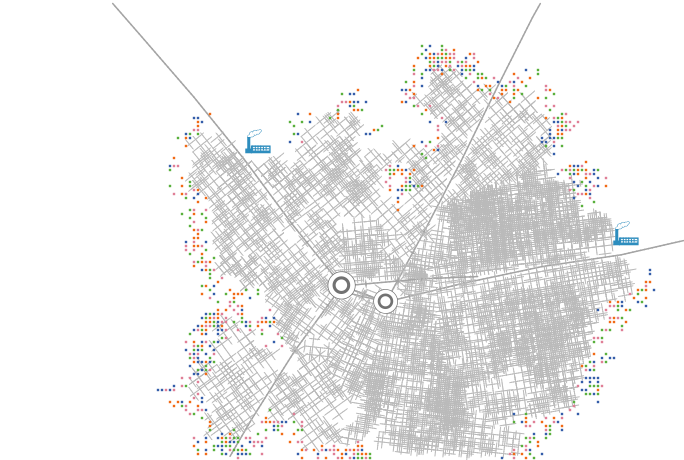
\includegraphics[width=0.33\textwidth]{Figures/Reproducibility/stdView}
\hfill
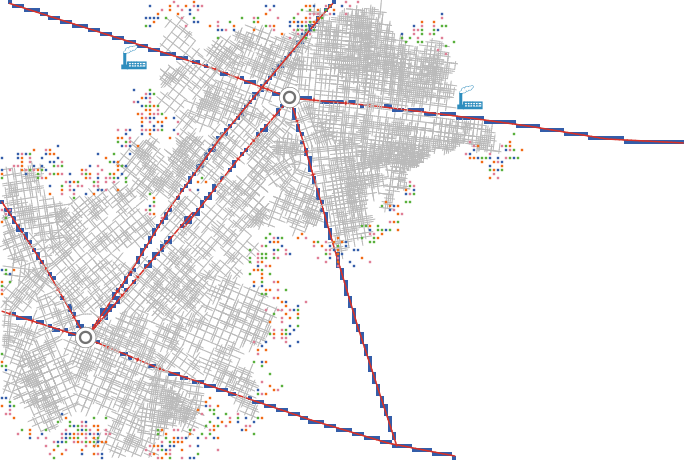
\includegraphics[width=0.33\textwidth]{Figures/Reproducibility/ViewRoads}
\hfill
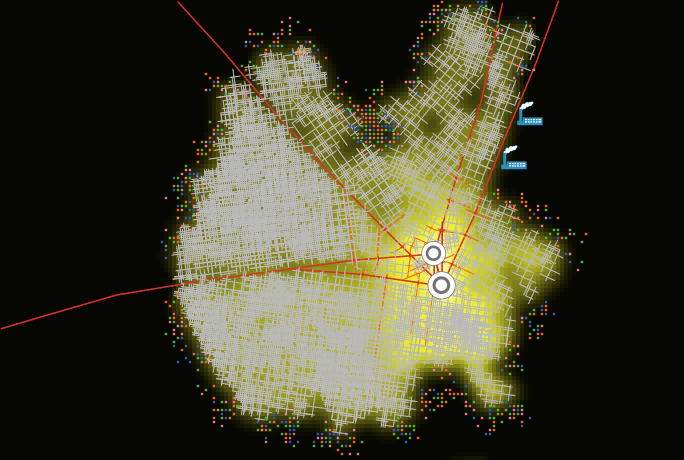
\includegraphics[width=0.33\textwidth]{Figures/Reproducibility/landValues_cityFinished}
\caption[Reproducibility and visualization][Reproductibilité et visualisation]{Example of simple improvement in visualization that can help understanding mechanisms implied in the model. \textit{Left: } Example of original output ; \textit{Middle: } Visualization of main roads (in red) and underlying patches attribution, suggesting possible implementation bias in the use of discretized trace of roads to track their positions ; \textit{Right: }Visualization of land values using a more readable color gradient. This step confirms the hypothesis, through the form of value distribution, that the morphogenesis step is an unnecessary detour to generate a random field for which simple diffusion method should provide similar results, as detailed in the paragraph on implementation.}{Exemple d'amélioration simple dans la visualisation qui peut aider à appréhender les mécanismes impliqués par le modèle. \textit{Gauche : } Exemple de sortie originale ; \textit{Centre : } Visualisation des routes principales (en rouge) et de l'attribution des patches sous-jacente, qui suggère de possibles biais d'implémentation dans l'utilisation de la trace discrete des routes pour garder trace de leur position ; \textit{Droite : } Visualisation des valeurs foncières en utilisant un gradient de couleur plus lisible. Cette étape confirme l'hypothèse, par la forme de la distribution des valeurs, que l'étape de morphogenèse est un détour non-nécessaire pour générer un champ aléatoire pour lequel des simples mécanismes de diffusion devrait fournir des résultats similaires, comme détaillé dans le paragraphe sur l'implémentation. \comment{(Florent) on ne peut pas comprendre ce que tu dis juste en regardant ces trois images. tu dois mieux accompagner le lecteur}}
\label{fig:example_tij_viz}
\end{figure}
%%%%%%%%%%%%%%%%%%%%%



\subsection{On the Need of Exactitude in Model Implementation}{Sur le besoin d'exactitude dans l'implémentation du modèle}

% Barthelemy paper, pb in model description/implementation
%  - test different analyses with possible biaises -


\bpar{
Possible divergences between model description in a paper and the effectively implemented processes may have grave consequences on the final reproducibility. The road network growth model given in~\cite{barthelemy2008modeling} is one example of such a discrepancy. A strict implementation of model mechanisms provide slightly different results than the one presented in the paper, and as source code is not provided we need to test different hypotheses on possible mechanisms added by the programmer (that seems to be a connexion rule to intersections under a certain distance threshold). Lessons that could be possibly drawn from this examples are 
\begin{itemize}
\item the necessity of providing source code
\item the necessity of providing architecture description along with code (if model description is in a langage too far from architectural specifications) in order to identify possible implementation biaises
\item the necessity of performing and detailing explicitly model explorations, that would in that case have helped to identify the implementation bias.
\end{itemize}
}{
Des divergences potentielles entre la description du modèle dans un article et les processus effectivement implémentés peut avoir des conséquences graves sur la reproductibilité finale. Le modèle de croissance du réseau routier donné dans~\cite{barthelemy2008modeling} est un exemple d'une telle discrépance. Une implémentation stricte des mécanismes du modèle produit des résultats légèrement différents de ceux présentés dans le papier, et comme le code source n'est pas fourni nous devons tester différentes hypothèses sur des mécanismes possibles ajoutés par le programmeur (qui semble être une règle de connexion aux intersections sous un certain seuil de distance). Des leçons qui peuvent éventuellement être tirées de cet exemple sont
\comment{(Florent) déjà dit non ?}[pas exactement même façon et pas même contexte]
\begin{itemize}
\item la nécessité de fournir le code source
\item la nécessité de fournir une description de l'architecture en même temps que le code (si la description du modèle est faite dans un langage trop loin de spécification architecturales) afin d'identifier des biais possibles d'implémentation
\item la nécessité de procéder à des explorations explicites du modèle et de les détailler, ce qui dans ce cas aurait permis d'identifier de possibles biais d'implémentation.
\end{itemize}
}



\bpar{
Making the last point mandatory may ensure a limited risk of scientific falsification as it is generally more complicated to fake false exploration results than to effectively explore the model. One could imagine an experiment to test the general behavior of a subset of the scientific community regarding reproducibility, that would consist in the writing of a false modeling paper in the spirit of~\cite{zilsel2015canular}, in which opposite results to the effective results of a given model are provided, without providing model implementation. A first bunch of test would be to test the acceptance of a clearly non-reproducible paper in diverse journals, possibly with a control on textual elements (using or not ``buzz-words'' associated to the journal, etc.). Depending on results, a second experiment may be tested with providing open source code for model implementation but still with false results, to verify if reviewers effectively try to reproduce results when they pretend to want the code (in reasonable computational power limits of course, HPC being not currently broadly available in Humanities).
}{
Rendre le dernier point obligatoire pourrait assurer un risque limité de falsification puisqu'il est généralement plus compliqué de falsifier des résultats d'exploration plutôt que d'explorer effectivement le modèle. \comment{(Florent) joint project.. : on n'a pas à connaitre tes side-projects}
 On pourrait imaginer une expérience pour tester le comportement général d'un sous-ensemble de la communauté scientifique au regard de la reproducibilité, qui consisterait en l'écriture d'un faux papier de modélisation
}


\subsection{Perspectives}{Perspectives}


\bpar{
Again, reproducibility and transparency is a non-negotiable feature of contemporaneous science, along with Open practices and Open Access. Too much examples (see a very recent one in experimental economics~\cite{camerer2016evaluating}) show in various disciplines the lack of reproducibility of experiments, that is a falsification of previous results or a result in itself. Falsification is a costly practice, and even if necessary~\cite{chavalarias2005nobel}, could be made more efficient through more transparency and direct reproducibility, increase therein the global workflow of science. We develop in parallel of this thesis various tools aimed to ease reproducibility, for which an overview is given in appendix~\ref{app:workflow}.
}{

}












%----------------------------------------------------------------------------------------

\newpage



\section{Big Data, Computation and Model Exploration}{Données Massives, Computation et Exploration des Modèles}






\subsection{For a cautious use of big data and computation}{Pour un usage raisonné des données massives et de la computation}

\bpar{
The so-called \emph{big data revolution} resides as much in the availability of large datasets of novel and various types as in the always increasing available computational power. Although the \emph{computational shift} (\cite{arthur2015complexity}) is central for a science aware of complexity and is undeniably the basis of future modeling practices in geography as \cite{banos2013pour} points out, we argue that both \emph{data deluge} and \emph{computational potentialities} are dangerous if not framed into a proper theoretical and formal framework. The first may bias research directions towards available datasets (as e.g. numerous twitter mobility studies) with the risk to disconnect from a theoretical background, whereas the second may overshadow preliminaries analytical resolutions essential for a consistent use of simulations. We argue that the conditions for most of results in this thesis are indeed the ones endangered by incautious big-data enthusiasm, concluding that a main challenge for future Geocomputation is a wise integration of novel practices within the existing body of knowledge.
}{
La soi-disante \emph{révolution des données massives} réside autant dans la disponibilité de grands jeux de données de nouveaux types variés, que dans la puissance de calcul potentielle toujours en augmentation. Même si le \emph{tournant computationnel} (\cite{arthur2015complexity}) est central pour une science consciente de la complexité et est sans douter la base des pratiques de modélisation futures en géographie comme \cite{banos2013pour} souligne, nous soutenons que à la fois le \emph{déluge de données} et les \emph{capacités de calcul} sont dangereuses si non cadrées dans un cadre théorique et formel propre. Le premier peut biaiser les directions de recherche vers les jeux de données disponibles %(comme par exemple les nombreuses étude de mobilité se basant sur twitter) % TODO find less rude examples, and of different types ?
 avec le risque de se déconnecter d'un fond théorique, tandis que le second peut occulter des résolutions analytiques préliminaires essentielles pour un usage cohérent des simulations. Nous avançons que les conditions pour la majorité des résultats dans cette thèse sont en effet ceux mis en danger par un enthousiasme inconsidéré pour les données massives, tirant la conclusion qu'un challenge majeur pour la géocomputation future est une intégration sage des nouvelles pratiques au sein du corpus existant de connaissances.
}


\bpar{
The computational power available seems to follow an exponential trend, as some kind of Moore's law. Both effective Moore's law for hardware, and improvement of softwares and algorithms, combined with a democratization of access to large scale simulation facilities, makes always more and more CPU time available for the social scientist (and to the scientist in general but this shift happened quite before in other fields, as e.g. CERN is leading in cloud computing and grid computation). About 10 years ago, \cite{gleyze2005vulnerabilite} concluded that network analysis, for the case of Parisian public transportation network, was ``limited by computation''. Today most of these analyses would be quickly done on a personal computer with appropriated software and coding: \cite{2015arXiv151201268L} is a witness of such a progress, introducing new indicators with a higher computational complexity, computed on larger networks. The same parallel can be done for the Simpop models: the first Simpop models at the beginning of the millenium~\cite{sanders1997simpop} were ``calibrated'' by hand, whereas \cite{cottineau2015modular} calibrates the multi-modeling Marius model and~\cite{schmitt2014half} calibrates very precisely the SimpopLocal model, both on grid with billions of simulations. A last example, the field of Space Syntax, witnessed a long path and tremendous progresses from its theoretical origins~\cite{hillier1989social} to recent large-scale applications~\cite{hillier2016fourth}.
}{
La puissance de calcul disponible semble suivre un tendance exponentielle, comme une sorte de loi de Moore. Grace à d'une part la loi de Moore effective pour le matériel, d'autre part l'amélioration des logiciels et algorithmes, conjointement avec une démocratisation de l'accès au infrastructures de simulation à grande échelle, permet à toujours plus de temps processeur d'être disponible pour le chercheur en sciences sociales (et pour le scientifique en général, mais cette mutation a déjà été opérée depuis plus longtemps dans d'autres domaines, puisque par exemple le CERN est à la pointe en terme de calcul distant et sur grille). Il y a environ une dizaine d'année, \cite{gleyze2005vulnerabilite} était forcé de conclure que les analyses de réseau, pour les transports publics parisiens, étaient ``limitées par le calcul''. Aujourd'hui la plupart des mêmes analyses seraient rapidement réglée sur un ordinateur personnel avec les logiciels et programmes appropriés : \cite{2015arXiv151201268L} est un témoin d'un tel progrès, introduisant des nouveaux indicateurs avec une plus grande complexité de calcul, qui sont calculés sur des réseaux à grande échelle. Le même parallèle peut être fait pour les modèles Simpop : les premiers modèles Simpop au début du millénaire~\cite{sanders1997simpop} étaient ``calibrés'' à la main, tandis que \cite{cottineau2015modular} calibre le modèle Marius en multi-modélisation et~\cite{schmitt2014half} calibre très précisément le modèle SimpopLocal, chacun sur la grille avec des milliards de simulations. Un dernier exemple, le champ de la \emph{Space Syntax}, a témoigné d'une longue route et de progrès considérables depuis ses origines théoriques~\cite{hillier1989social} jusqu'à ses récentes applications à grande échelle~\cite{hillier2016fourth}.
}



\bpar{
Concerning the new and ``big'' data available, it is clear that always larger dataset are available and always newer type of data are available. Numerous examples of fields of application can be given. For example, mobility can now be studied from various entries, such as new data from smart transportation systems~\cite{o2014mining}, from social networks~\cite{frank2014constructing}, or other more exotic data such as mobile phone data~\cite{de2016death}. In an other spirit, the opening of ``classic'' datasets (such as city dashboards, open data government initiatives) should allow ever more meta-analyses. New ways to do research and produce data are also raising, towards more interactive and crowd-sourced initiatives. For example, \cite{2016arXiv160606162C} describes a web-application aimed at presenting a meta-analysis of Zipf's law across numerous datasets, but in particular features an upload option, where the user can upload its own dataset and add it to the meta-analysis. Other applications allow interactive exploration of scientific literature for a better knowledge of a complex scientific landscape, as~\cite{cybergeo20} does.
}{
Concernant les nouvelles données ``massives'' qui sont disponibles, il est clair que des quantités toujours plus grandes et des types toujours nouveaux sont disponibles. De nombreux exemples de champs d'application peuvent être donnés. La mobilité en est typique, puisque étudiée selon divers points de vue, comme les nouvelles données issues des systèmes de transport intelligents~\cite{o2014mining}, des réseaux sociaux~\cite{frank2014constructing}, ou des données plus exotiques comme des données de téléphonie mobile~\cite{de2016death}. Dans un autre esprit, l'ouverture de jeux de données ``classiques'' (comme les applications synthétiques urbaines, les initiatives gouvernementales pour les données ouvertes) devrait pouvoir toujours plus de méta-analyses. De nouvelles façon de pratiquer la recherche et produire des données sont également en train d'émerger, vers des initiatives plus interactives et venant de l'utilisateur. Ainsi, \cite{2016arXiv160606162C} décrit une application web ayant pour but de présenter une méta-analyse de la loi de Zipf sur de nombreux jeux de données, mais en particulier inclut une option de dépôt, à travers laquelle l'utilisateur peut télécharger sont propre jeu de données et l'inclure dans la méta-analyse. D'autres applications permettent l'exploration interactive de la littérature scientifique pour une meilleure connaissance d'un horizon scientifique complexe, comme~\cite{cybergeo20} fait.
}


\bpar{
As always the picture is naturally not as bright as it seems to be at first sight, and the green grass that we try to go eating in the neighbor's field quickly turns into a sad reality. Indeed, the purpose and motivation are fuzzy and one can get lost. Some examples speaks for themselves. \cite{barthelemy2013self} introduces a new dataset and rather new methods to quantify road network evolution, but the results, on which the authors seem to be astonished, are that a transition occurred in Paris at the Haussmann period. Any historian of urbanism would be puzzled by the exact purpose of the paper, as in the end a vague and bizarre feeling of reinventing the wheel floats in the air. The use of computation can also be exaggerated, and in the case of agent-based modeling it can be illustrated by the example of~\cite{axtell2016120}, for which the aim at simulating the system at scale 1:1 seems to be far from initial motivations and justifications for agent-based modeling, and may even give arguments to mainstream economists that denigrate easily ABMS. Other anecdotes raise worries: \cite{robin_cura_2014_11415} is a web application that wastes computational ressources to simulate Gaussian distributions for a Gibrat model in order to compute their mean and variance, that are input parameters of the model. It basically checks the Central Limit Theorem, which is a priori well accepted among most scientists. Otherwise, the full distribution given by a Gibrat model is theoretically known as it was fully solved e.g. by \cite{gabaix1999zipf}. Recently on the French speaking diffusion list \emph{Geotamtam}, a sudden rush around \emph{Pokemon Go} data seemed to answer more to an urgent unexplained need to exploit this new data source before anyone else rather than an elaborated theoretical construction. Simple existing accurate datasets, such as historical cities population (for France the Pumain-INED database for example), are far from being fully exploited and it may be more important to focus on these already existing classic data. One must also be aware of the possible misleading applications of some results: \cite{louail2016crowdsourcing} makes a very good analysis of potential redistribution of bank card transactions within a city, but pushes the results as possible basis for social equity policy recommandation by acting on mobility, forgetting that urban form and function are coupled in a complex way and that moving transactions from one place to the other involves far more complex processes than policies (even in a country like China were policies are actually enforced with a hand of steel).
}{
Comme toujours la situation n'est naturellement pas aussi idyllique qu'elle semble être au premier abord, et l'herbe verte du pré du voisin que nous pouvons être tentés d'aller brouter se transforme rapidement en un triste fumier. En effet, les objectifs et motivations sont flous et on peut facilement s'y perdre. Des illustrations parleront d'elles-même. \cite{barthelemy2013self} introduit un nouveau jeu de données et des méthodes relativement nouvelles pour quantifier l'évolution du réseau de rues, mais les résultats, sur lesquels les auteurs semblent s'étonner, sont qu'une transition a eu lieu à Paris à l'époque d'Haussmann. Tout historien de l'urbanisme s'interrogerait sur le but exact de l'étude, puisque à la fin un sentiment étrange de réinvention de la roue flotte dans l'air. L'utilisation des ressources de calcul peut également être exagéré, et dans le cas de la modélisation multi-agent, on peut citer~\cite{axtell2016120}, pour lequel l'objectif de simuler le système à l'échelle 1:1 semble être loin des motivations et justifications originelles de la modélisation agent, et pourrait même donner des arguments aux économistes \emph{mainstream} qui dénigrent facilement les ABMS. D'autres anecdotes peuvent inquiéter : %\cite{robin_cura_2014_11415} % do not cite this shit
est une application web qui gâche des ressources de calcul  pour simuler des distributions Gaussiennes afin de calculer pour un modèle de Gibrat, afin de calculer leur moyenne et variance, qui sont des paramètres d'entrée du modèle. En résumé, cela revient à vérifier le Théorème de la Limite Centrale, qui est a priori assez accepté par la plupart des scientifiques. D'autre part, la distribution complète donnée par un modèle de Gibrat est entièrement connue théoriquement comme résolu e.g. par~\cite{gabaix1999zipf}. Récemment, sur la liste de diffusion de géographie francophone \emph{Geotamtam}, un soudain engouement autour des données issues de \emph{Pokemon Go} a semblé répondre plus à un besoin urgent et inexpliqué d'exploiter cette source de données avant tous les autres, plutôt qu'à des considérations théoriques élaborées. Des jeux de données existant et précis, comme la population historiques des villes (pour la France la base Pumain-INED par exemple), sont loin d'être entièrement exploités et il pourrait être plus pertinent de se concentrer sur ces jeux de données classiques qui existent déjà. De même, il faut être conscient des possibles applications de résultats basée sur des malentendus : \cite{louail2016crowdsourcing} fait une très bonne analyse de la redistribution potentielle des transactions de carte bancaire au sein d'une ville, mais présente les résultats comme la base possible de recommandations de politiques pour une équité sociale en agissant sur la mobilité, oubliant que la forme et les fonctions urbaines sont couplés de manière complexe et que déplacer des transactions d'un endroit à un autre implique des processus bien plus complexes que des régulations directes (même dans un pays comme la Chine ou les régulations sont effectivement mise en place et imposées d'une main de fer).
}




\bpar{
Our main claim here is that the computational shift and simulation practices will be central in geography, but may also be dangerous, for the reasons illustrated above, i.e. that data deluge may impose research subjects and elude theory, and that computation may elude model construction and solving. A stronger link is required between computational practices, computer science, mathematics, statistics and theoretical geography. Theoretical and Quantitative Geography is at the center of this dynamic, as it was its initial purpose that seems forgotten in some cases. It implies the need for elaborated theories integrated with conscious simulation practices. In other words we can answer complementary naive questions that have however to be tackled one and for once. If a theory-free quantitative geography would be possible, the answer if naturally no as it is close to the trap of black-box data-mining analysis. Whatever is done in that case, the results will have a very poor explanatory power, as they can exhibit relations but not reconstruct processes. On an other hand, the possibility of a purely computational quantitative geography is a dangerous vision: even gaining three orders of magnitudes in computational power does not solve the dimensionality curse. In our work here, without theory, we would not know which objects, measures and properties to look at (e.g. multi-scale and dynamical nature of processes), and without analytics, it would be sometimes difficult to draw conclusions from empirical analysis. Nothing is really new here but this position has to be stated and stood up, precisely because our work will use this kind of tools, trying to advance on a thin and fragile edge, with the void of the unfunded theoretical charlatanism on one side and the abyss of the technocratic blind drowning in foolish amounts of data. More than ever we need simple but powerful and funded theories {\`a}-la-Occam~\cite{batty2016theoretical}, to allow a wise integration of new techniques into existing knowledge.
}{
Notre principal argument est que le tournant computationnel et les pratiques de simulation seront centrales en géographie, mais peuvent également être dangereux, pour les raisons illustrées ci-dessus, i.e. que le déluge de données peut imposer les sujets de recherche et occulter la théorie, et que la computation peut éluder la construction et la résolution de modèles. Un lien plus fort est nécessaire entre les pratiques de calcul, l'informatique, les mathématiques, les statistiques et la géographie théorique. La Géographie Théorique et Quantitative est au centre de cette dynamique, puisqu'il s'agit de sa motivation initiale principale qui semble oubliée dans certains cas. Cela implique un besoin de recherche de théorie élaborées intégrées avec des pratiques de simulation conscientes. En d'autres mots, on peut répondre à des questions naïves complémentaires qui ont toutefois besoin d'être traitées une bonne fois pour toutes. Si une géographie quantitative libérée de la théorie serait possible, la réponse est naturellement non puisque cela se rapproche du piège de la fouille de données par boîte noire. Quoi qu'il soit fait par cette approche, les résultats auront un pouvoir explicatif très faible, puisqu'ils pourront mettre en valeur des relations mais pas reconstruire des processus. D'autre part, la possibilité d'une géographie quantitative purement basée sur le calcul est une vision dangereuse : même le gain de trois ordres de grandeur dans la puissance de calcul disponible ne résout pas le sort de la dimension. Dans notre travail ici l'absence de théorie impliquerait de ne pas connaitre les objets, mesures et propriétés à étudier (e.g. le caractère multi-scalaire ou dynamique des processus), et sans résolutions analytiques, il serait souvent difficile de tirer des conclusions à partir des analyses empiriques. Rien n'est vraiment nouveau ici mais cette position doit être affirmée et tenue, précisément car notre travail se base sur ce type d'outils, essayant d'avancer sur une arête fine et fragile, avec d'un côté le vide du charlatanisme théorique infondé et de l'autre l'abîme de l'overdose technocratique dans des quantités de données folles. Plus que jamais on a besoin de théories simples mais fondées et puissantes {\`a}-la-Occam~\cite{batty2016theoretical}, pour permettre une intégration saine des nouvelles techniques au sein des connaissances existantes.
}


 
% multi-modeling and model families (see Cottineau, Rey and Reuillon presentation) as one way to do that ?

% Interdisciplinarity (and Nexus ?!) necessary to achieve that.













%----------------------------------------------------------------------------------------


\newpage


%  section : synthetic data control - introduces rochebrune paper, feasible correlation space etc, and forthcoming applications ?


\section{Statistical Control on Initial Conditions by Synthetic Data Generation}{Contrôle statistique pour les conditions initiales par génération de données synthétiques}

\subsection{Context}{Contexte}


\bpar{
When evaluating data-driven models, or even more simple partially data-driven models involving simplified parametrization, an unavoidable issue is the lack of control on ``underlying system parameters'' (what is a ill-defined notion but should be seen in our sense as parameters governing system dynamics). Indeed, a statistics extracted from running the model on enough different datasets can become strongly biased by the presence of confounding in the underlying real data, as it is impossible to know if result is due to processes the model tries to translate or to a hidden structure common to all data.
}{
Lors de l'évaluation de modèle basés sur les données, \comment{(Florent)  data driven models : sens de cette expression ?} ou même de modèle plus simples partiellement basés sur les données impliquant une paramétrisation simplifiée, une issue inévitable est le manque de contrôle sur les ``paramètres implicites du systèmes'' (ce qui n'est pas une notion stricte mais doit être vu dans notre sens comme les paramètres régissant la dynamique). En effet, une statistique issue d'executions du modèle sur un nombre suffisamment grand de jeu de données peut devenir fortement biaisé par la présence de \emph{confunding} dans les données réelles sous-jacentes, comme il est impossible de savoir si les résultats sont dus aux processus que le modèle cherche à traduire ou à une structure commune à toutes les données.
\comment{(Florent) a quelle question cherches-tu ici à répondre ?}
}


%Let illustrate the issue with a simple example.

We formalize briefly a proposition of method that would allow to add controls on meta-parameters, in the sense of parameters driving the represented system at a higher temporal and spatial scale, for a model of simulation. We make the hypothesis that such method is valid under constraints of disjonction for scales and/or ontologies between the model of simulation and the domain of meta-parameters.


\subsection{Description}{Description}

An advanced knowledge of the behavior of computational models on their parameter space is a necessary condition for deductions of thematic conclusions \comment{(Florent) pas nécessaire si les comportements sont bien calibrés par des observations dans le monde réel, il n'est pas besoin d'une compréhension si fine du modèle}
 or their practical application~\cite{banos2013pour}. But the choice of varying parameters is always subjective, as some may be fixed by a real-world parametrization, or other may be interpreted as arbitrarily fixed initial conditions. It raises methodological and epistemological issues for the sensitivity analysis, as the scope of the model may become ill-defined. \comment{(Florent) sens ?}

Let consider the concrete example of the Schelling Segregation model~\cite{schelling1971dynamic}. \comment{(Florent) Schelling hors sujet ?}
One of its crucial features on which the literature has been rather controversial is the influence of the spatial structure of the container on which agents evolve.%~(\textit{Biblio Marion}). 
 The thematic aim of the project developed in~\cite{cottineau2015revisiting} is to clarify this point through a systematic model exploration. A methodological contribution is the construction of a framework allowing the analysis of the sensitivity of models to \emph{meta-parameters}, i.e. to parameters considered as fixed initial conditions (e.g. the spatial structure for the Schelling model), or to parameters of another model generating an initial configuration%, as detailed in Fig.~\ref{} \textit{[insert scheme describing the approach]}, 
 yielding thus a \emph{simple coupling} between models (serial coupling). The benefits of such an approach are various but include for example the knowledge of model behavior in an extended frame, the possibility of statistical control when regressing model outputs, a finer exploration of model derivatives than with a naive approach. Some remarks can be made on the approach :
\begin{itemize}
\item What knowledge are brought by adding the upstream model, rather than for example in the Schelling case exploring a large set of initial geometries ? 

$\rightarrow$ \textit{to obtain a sufficiently large set of initial configuration, one quickly needs a model to generate them ; in that case a quasi-random generation followed by a filtering on morphological constraint will be a morphogenesis model, which parameters are the ones of the generation and the filtering methods. Furthermore, as detailed further, the determination of the derivative of the downstream model is made possible by the coupling and knowledge of the upstream model.}
\comment{(Florent) est-ce important pour la thèse ?}


\item Statistical noise is added by coupling models

$\rightarrow$ \textit{Repetitions needed for convergence are indeed larger as the final expectance has to be determined by repeating on the first times the second model ; but it is exactly the same as exploring directly many configuration, to obtain statistical robustness in that case one must repeat on similar configurations.}

\item Complexity is added by coupling models

% check Varenne citation
$\rightarrow$ \textit{In the sense of Varenne~\cite{varenne2010framework} , coupling is simple and no complexity is thus added.}
\end{itemize}
 
%\paragraph{Context}

%Let $M_{m}$ a stochastic model of simulation, which inputs are to simplify initial conditions $D_0$ and parameters $\vec{\alpha}$, and output $M_{m}\left[\vec{\alpha},D_0\right](t)$ at a given time $t$. We assume that it is partially data-driven in the sense that $D_0$ is supposed to represent a real situation at a given time, and model performance is measured by the distance of its output at final time to the real situation at the corresponding time, i.e. error function is of the form $\norm{\Eb{\vec{g}(M_{m}\left[\vec{\alpha},D_0\right](t_f))}-\vec{g}(D_f)}$ where $\vec{g}$ is a deterministic field corresponding to given indicators.

%\paragraph{Position of the Problem}

%Evaluating the model on real data is rapidly limited in control possibilities, being restricted to the search of datasets allowing natural control groups. Furthermore, statistical behaviors are generally poorly characterized because of the small number of realizations. Working with synthetic data first allows to solve this issue of robustness of statistics, and then gives possibilities of control on some ``meta-parameters'' in the sense described before.




%%%%%%%%%%%%%%%%%%%%
\subsection{Formal Description}{Description Formelle}

%\subsubsection{Deterministic Formulation}

One has the composition of the derivative along the meta-parameter

\[
\partial_{\alpha}\left[M_u \circ M_d\right] = \left(\partial_{\alpha} M_u \circ M_d \right)\cdot \partial_{\alpha} M_d
\]

$\rightarrow$ \textit{the sensitivity of the downstream model (Schelling) can be determined by studying the serial coupling and the upstream model ; thematic knowledge : sensitivity to an implicit meta-parameter ; and computational gain : generation of controlled differentiates in the ``initial space'' is quasi impossible.}

%\subsubsection{Stochasticity}

The question of stochasticity in simply coupled models causes no additional issue as $\Eb{X}=\Eb{\Eb{X|Y}}$. It naturally multiplies the number of repetition needed for convergence what is the expected behavior.








%----------------------------------------------------------------------------------------


\newpage




\section{Epistemological Positioning}{Positionnement Epistémologique}\label{sec:epistemo-position}





% Pour une science anarchiste (Feyerabend) ; compatibilité avec le Perspectivisme de Giere et pourquoi celui-ci est particulièrement adapté aux paradigmes de la complexité ; multiplicité des lectures de la thèse (voir annexe réflexivité, au delà d'une lecture linéaire)










